\chapter{Construção da Ferramenta~\label{chp:construção-da-ferramenta}}

A ferramenta construída neste trabalho, nomeada \textit{\textbf{tjscraper}},
foi produzida para ser capaz de extrair com qualidade
satisfatória~\todofootnote{}{(Definir ``qualidade satisfatória'' --- em resumo:
um formato que dê de usar os dados para alguma coisa e que não seja ``grego''
para alguém que não seja da área)} os dados especificamente do TJ do Rio de
Janeiro (TJ-RJ). As estratégias empregadas, portanto, levam em conta acessos
que todos os acessos serão ao TJ-RJ, ainda que visando a possibilidade de serem
aplicadas às páginas dos TJs dos demais estados.

\section{Ferramentas utilizadas~\label{section:ferramentas-utilizadas}}

\textcolor{blue}{--->> O que estás propondo para descrição de ferramentas
(Scrapy e SQLLite) será um pequeno parágrafo de uma Seção chamada "Ferramentas
utilizadas" no capítulo de construção da ferramenta. Não vais descrever nenhuma
delas com detalhes, pois são ferramentas simplesmente usadas para contruíres
teu trabalho. Isso não se detalha porque não são "conceitos". Ferramentas mudam
de versão, saem de linha, ficam obsoletas, perdem valor, etc, portanto, não se
descrevem em detalhes.}

\todo{%
    Esta seção deve ser uma descrição das ferramentas mais relevantes que foram
    \textit{utilizadas} no trabalho, i.e. as dependências (bibliotecas,
    linguagem de programação).
}
\begin{todolist}
    \item Scrapy
    \item SQLite
    \item \ldots
\end{todolist}

\section{Organização geral}

\begin{todolist}
    \item Diagramar módulos;
\end{todolist}

A ferramenta foi projetada como uma biblioteca de \textit{software} acompanhada
de duas interfaces de usuário~\footnote{Neste ponto, ``usuário'' refere-se a
alguém que não esteja utilizando a ferramenta como uma biblioteca de software,
e sim como aplicação.}: uma aplicação de Interface de Linha de Comando
(\textit{ILC}\footnote{Comumente referenciado com a sigla em inglês ``CLI'', de
``Command Line Interface''.} e uma aplicação de servidor Web.

A ILC tem como objetivo permitir o uso de boa parte dos diferentes recursos da
biblioteca em um terminal para a execução tarefas pontuais, como exibir
informações sobre estado atual da \textit{cache}, iniciar um processo de
extração, ou mesmo iniciar uma instância de servidor Web da ferramenta para
fins de desenvolvimento.

O servidor Web é destinado ao usuário que queira uma interface de simples
acesso e uso da ferramenta, primariamente focando na obtenção de dados dos TJs
com os recursos que não estejam disponíveis nas páginas oficiais dos TJs
(descritos na~\todo{Referenciar Seção}), tendo em mente como público alvo
jornalistas.

\section{Estratégias de extração}

O TJ-RJ possui rotas e subdomínios que dão acesso aos mesmos dados por formatos
de apresentação diferentes. Foram elaboradas estratégias para extrair dados da
rota que os fornece em formato HTML~\todofootnote{}{link da rota HTML},
conhecida antes da produção efetiva da ferramenta, e da que os fornece em
formato JSON~\todofootnote{}{link da rota JSON}, encontrada durante o processo
de produção e portanto implementada posteriormente. O formato HTML é
apresentado como uma página de consulta para um usuário comum, enquanto o
formato JSON é um conjunto de rotas que implementam uma API Web.

Para a produção desta ferramenta não foi encontrada uma forma de se obter todos
os processos de maneira direta. A estratégia, então, foi exaurir as
possibilidades de valores de entrada de algum dos tipos de busca disponíveis
nos portais do TJ-RJ. Analisando as dificuldades existentes em cada um dos
tipos (\Cref{tbl:dificuldades-tipos-de-busca}), foi escolhido o campo de busca
por número do processo por conta do domínio de valores válidos ser limitado e
conhecido: números de processos são dados seguindo os formatos numéricos fixos
\textbf{unificado} e \textbf{antigo}, respectivamente
``NNNNNNN-NN.AAAA.8.19.NNNN'' e ``AAAA.NNN.NNNNNN-N'' em que ``AAAA'' é o ano
de criação do documento do processo e cada ``N'' é um dígito de 0 a 9, logo é
possível encontrar todos os processos apenas fixando o ano e testando
diferentes combinações para os demais dígitos.

\begin{table}[htb]
    \centering
    \begin{tabular}{lp{0.65\textwidth}}
        \toprule
        Tipo de busca & Dificuldades \\
        \midrule
        Por Número & Número alto de combinações possíveis (para cada ano, $10^{13}$ para numeração unificada ou $9 \times 10^{10}$ para numeração antiga). \\
        Por Nome & Inviável. Demanda conhecer todos os nomes existentes em processos. \\
        Por OAB & Sem garantia de cobertura completa. \\
        Por Nome do Advogado & Inviável. Demanda conhecer todos os nomes existentes em processos. \\
        Por CPF / CNPJ & Número alto de combinações possíveis (em um sequenciamento ingenuo, $10^{11}$ para CPF e $10^{14}$ para CNPJ). \\
        Por Protocolo & Sem garantia de cobertura completa. \\
        Por Sentença & Sem garantia de cobertura completa. \\
        \bottomrule
    \end{tabular}
    \caption{%
        Dificuldades encontradas para se exaurir as possibilidades de valores
        de entrada para cada um dos campos de busca permitidos pelo TJ-RJ.
    }
    \label{tbl:dificuldades-tipos-de-busca}
\end{table}

\todo{%
    Sobre o formato numérico antigo: trocar para o \textbf{unificado} no
    código, pois o antigo varia conforme vara/etc.
}

\review{Outros campos, como nome das partes por exemplo, possuem uma
abrangência de valores muito grande e difícil de se conhecer em sua totalidade
ou, nos casos como a busca por Sentença, não são capazes de, mesmo exauridas
todas as combinações de valores de entrada, dar acesso a todos os processos
registrados.}

\review{A numeração dos processos não é sequencial}

\subsection{Estratégia inicial: extração HTML}

\begin{todolist}
    \item Ressaltar dificuldades com páginas diferentes, fornecendo links para
          exemplos --- para fins de reprodutibilidade, o link será uma cópia
          para um .html salvo no repositório do código da ferramenta, na pasta
          de ``samples'' (amostras);
\end{todolist}

\review{Para extração das rotas do TJ-RJ que fornecem seu conteúdo no formato
HTML, a estratégia é semelhante a reproduzir o acesso de um usuário comum ao
efetuar uma busca. A rota de Consultas Processuais
unificada~\footnote{\url{http://www4.tjrj.jus.br/ConsultaUnificada/consulta.do}}
exibe uma página que permite a busca por processos por ambos os tipos de
numeração.}

Os resultados de consulta processual do TJ-RJ em HTML são os das requisições
feitas ao subdomínio \url{ww4.tjrj.jus.br}. A estratégia de extração dos
processos que ele disponibiliza é aproveitar que a identificação de qual
processo está sendo visualizado pode ser feita através do parâmetro de URL
\texttt{numProcesso}, cujo valor é o número do processo na numeração antiga,
efetuando requisições para a mesma URL variando apenas esse parâmetro com um
número de processo. Cada requisição pode retornar uma página de processo
válido, inexistente~\footnote{Exemplo de URL de processo inexistente:
\url{http://www4.tjrj.jus.br/consultaProcessoWebV2/consultaProc.do?numProcesso=2020.004.015548-9}},
de numeração inválida~\footnote{Exemplo de URL de processo inválido:
\url{http://www4.tjrj.jus.br/consultaProcessoWebV2/consultaMov.do?numProcesso=0}}
ou de Captcha (caso esteja fora do horário noturno~\todofootnote{}{Definir
horário noturno em alguma seção anterior.}).

Por não se tratar de um formato de descrição de dados (contrastando com JSON),
a extração de páginas HTML demanda o uso de ferramentas especializadas que
permitam a definição de padrões de como localizar dos campos desejados e
separar seus respectivos valores. Por resolver essa demanda com recursos que
visam facilitar tarefas comuns em raspagem de dados, foi escolhida a biblioteca
Scrapy~\cite{lib:scrapy}. Assim, os passos da extração foram determinados como:

\begin{enumerate}
    \item Dado um intervalo de números de processos (no formato unificado ou
        antigo), as URLs correspondentes a cada um dos valores nele são
        montadas e repassadas para uma \textit{spider} do Scrapy;
    \item Cada URL passada irá eventualmente, em alguma ordem, chamar o método
        \texttt{parse} da \textit{spider}, e nele é extraído o conteúdo de uma
        página seguindo os passos~\label{step-1}:

        \begin{enumerate}
            \item Identificar se a página é de um processo inválido,
                inexistente ou se há a exigência de preenchimento de um
                textit{captcha}.
            \item Caso seja um processo válido, buscam-se na página os campos
                desejados utilizando
        \end{enumerate}
\end{enumerate}

Para os passos do~\cref{step-1}, utilizou-se a especificação~\cite{spec:xpath}
suportada nativamente pelo Scrapy para a busca dos padrões de resultado e de
campos desejados no HTML da página.

\todo{Especificar XPath para páginas de erro.}

\newcommand{\urlProcValido}{\url{%
    http://www4.tjrj.jus.br/consultaProcessoWebV2/consultaProc.do?numProcesso=2021.004.015548-9
}}

Uma página de resultado da consulta pública do subdomínio ww4 do TJ-RJ para um
número de processo válido~\footnote{\urlProcValido}
(\Cref{fig:exemplo-pagina-ww4}) apresenta os campos dos dados do processo em
uma \textit{tag} HTML \texttt{<table>}, de forma que cada linha visual
corresponde a uma \textit{tag} \texttt{tr} composta por duas \textit{tags}
\texttt{td}: uma para o nome do campo e outra para o valor
(\Cref{cod:html-assunto}). Assim, um campo ``A'' pode ser encontrado procurando
por uma \texttt{td} cujo conteúdo seja ``A:'', e o valor é o próximo vizinho em
relação à hierarquia do HTML da página. A expressão XPath que representa esse
padrão é utilizada na função \mintinline{python}{extract_field(field_text)}
(\Cref{cod:extract_field}), que extrai o valor de um campo arbitrário em uma
resposta contendo uma página HTML conforme a seguinte ideia:

\begin{enumerate}
    \item \texttt{//}: Define que o item buscado pode estar em qualquer ponto
        do documento. Uma busca genérica dessa forma evita que pequenas
        variações na hierarquia HTML da página prejudiquem a busca.
    \item \texttt{td[text()='TEXTO:']}: Busca e seleciona um item da
        \textit{tag} \texttt{<td>} que tenha como conteúdo exatamente a
        \textit{string} ``TEXTO:''.
    \item \texttt{/following-sibling::td}: Se foi encontrado o item, então será
        seleciona o próximo vizinho de mesmo nível hierárquico que seja da
        \textit{tag} \texttt{<td>}.
    \item \texttt{/text()}: Desse item vizinho, captura-se o conteúdo dele como
        \textit{string}. Por ser o último item do XPath, então esse será o
        valor retornado pela busca.
\end{enumerate}


\begin{figure}[H]
    \centering{}
    \includegraphics{img/exemplo-resultado-consulta-publica-1.png}
    \caption{%
        Página de resultado da consulta pública para o processo válido de
        número 2021.003.015548-9 (numeração antiga).
    }
    \label{fig:exemplo-pagina-ww4}
\end{figure}

\begin{listing}
    \centering{}
    \begin{minted}[autogobble,breaklines]{html}
        <tr>
          <td class="info" valign="top" nowrap="nowrap">Assunto:</td>
          <td valign="top">
            Incapacidade Laborativa Permanente / Auxílio-Acidente (Art. 86) / Benefícios em Espécie
          </td>
        </tr>
    \end{minted}
    \caption{Código HTML do campo ``Assunto:'' presente na~\Cref{fig:exemplo-pagina-ww4}.}
    \label{cod:html-assunto}
\end{listing}

\begin{listing}[htb]
    \centering{}
    \begin{minted}[breaklines]{python}
        def extract_field(response: Response, field_text: str) -> str:
            field_xpath = f"//td[text()='{field_text}:']/following-sibling::td/text()"
            return response.xpath(field_xpath).get().strip()
    \end{minted}
    \caption{%
        Código da função responsável pela extração de um campo em uma resposta
        de uma requisição a uma página de visualização de processo.
    }
    \label{cod:extract_field}
\end{listing}

A extração de todos os campos desejados compõe os dados de um processo, que
então é exportado como uma linha adicional em um arquivo no
formato~\cite{spec:jsonlines}. Ao final de uma varredura por um intervalo de
número de processos, o arquivo contém os dados de todos os processos processos
dele.

\subsection{Estratégia alternativa: varredura com API JSON}

\begin{todolist}
    \item Iniciar descrevendo a relação entre parâmetros de busca da busca HTML
          e as rotas como \texttt{/por-numero/}.
    \item Expor sobre a existência de múltiplos sub-domínios do TJ-RJ;
    \item Complementar com a falta de documentação da API do TJ-RJ (forma de
          operação descoberta na base de tentativa e erro);
    \item Explicar rapidamente sobre a filtragem dos campos;
\end{todolist}

\urldef\urlConsultaJson\url{https://www3.tjrj.jus.br/consultaprocessual/#%2Fconsultapublica%23porNumero=}

No subdomínio \url{ww3.tjrj.jus.br}, há uma página de
busca~\footnote{\urlConsultaJson} semelhante à oferecida no subdomínio
\url{ww4.tjrj.jus.br}, também fornecendo os dados em HTML. Porém, em vez de o
servidor responder com o HTML pronto para o lado cliente renderizar, neste
subdomínio o cliente envia uma requisição AJAX para o uma API do
servidor~\footnote{\url{https://www3.tjrj.jus.br/consultaprocessual/api/processos/por-numero/publica}}
que responde com um objeto JSON e então o HTML é atualizado no lado cliente de
forma dinâmica. A estratégia então nesse caso passa a ser trivial: a partir do
número de um processo, enviar uma requisição para a tal API e, com os dados de
um processo em JSON, basta investigar quais os campos retornados, filtrar os de
interesse e exportar para o arquivo~\cite{spec:jsonlines}.

Por não ter sido encontrada uma documentação oficial, o funcionamento e
respostas dadas pela API foram descobertos a partir de tentativa e erro. A API
responde com dados de um processo através de requisições POST utilizando
\textit{query strings} para especificar os parâmetros de busca, cujos tipos de
resultados encontrados durante a construção desta ferramenta estão expostos
na~\Cref{tbl:respostas-ww3}.

\begin{table}[htb]
    \tiny
    \centering
    \begin{tabular}{lp{0.6\textwidth}}
        \toprule
        \textit{Query String} & Resposta (JSON) \\
        \midrule
        \texttt{tipoProcesso=1\&codigoProcesso=0} & \mintinline{json}{["O processo informado não foi encontrado."]} \\
        \texttt{tipoProcesso=1\&codigoProcesso=abc} & \mintinline{json}{["Número do processo inválido."]} \\
        \texttt{tipoProcesso=1\&codigoProcesso=2021.001.140006-4} & \mintinline{json}{{"codProc": "2021.001.140006-4", [...]}} \\
        Qualquer (em período noturno) & \begin{minipage}{0.6\textwidth}
            \begin{minted}[autogobble,breaklines]{json}
{"status": 412, "mensagem": "Erro de validação do Recaptcha. Tente novamente."}
            \end{minted}
        \end{minipage}
        \\
        \bottomrule
    \end{tabular}
    \caption{%
        Respostas dadas pela API do \url{ww3.tjrj.jus.br} conforme diferentes valores na \textit{query string}.
    }
    \label{tbl:respostas-ww3}
\end{table}

A resposta em formato JSON para busca por número, em caso de um número válido
de um processo existente, é um único objeto em que cada campo do processo
possui uma chave correspondente no objeto. Essas chaves são pré-definidas e
algumas opcionais, então para a extração dos campos desejados basta uma
consulta simples a elas no objeto seguindo a relação exposta
na~\Cref{tbl:relação-chaves-campos-json}.

Apesar de esta estratégia se demonstrar mais fácil e eficiente de se
implementar e utilizar, ambas foram mantidas na ferramenta para a extração de
dados em TJs que não possuam uma API JSON como a do TJ-RJ.

\begin{table}[htb]
    \tiny
    \centering
    \begin{tabular}{llp{0.4\textwidth}}
        \toprule
        Campo desejado & Chave no objeto JSON & Valor de exemplo \\
        \midrule
        Assunto & \texttt{"txtAssunto"} & \texttt{"Furto  (Art. 155 - CP)"} \\
        Número do Processo (Num. Antiga) & \texttt{"codProc"} & \texttt{"2021.001.140006-4"} \\
        Número do Processo (Num. Unificada) & \texttt{"codCnj"} & \texttt{"0158400-75.2021.8.19.0001"} \\
        Data de distribuição & \texttt{"dataDis"} & \texttt{"14/07/2021"} \\
        Unidade Federativa (UF) & \texttt{"uf"} & \texttt{"RJ"} \\
        Advogados (Nome, Número da OAB, ) & \texttt{"advogados"} & \texttt{[\{"nomeAdv": "DEFENSOR PÚBLICO", "numOab": "0"\}, ...]} \\
        Cidade & \texttt{"cidade"} & \texttt{"Rio de Janeiro"} \\
        Personagens (Autor, Autor do Fato, \ldots) & \texttt{"personagens"} & \texttt{[\{"codPers": "29760922", "nome": "MINISTERIO PUBLICO DO ESTADO DO RIO DE JANEIRO", "codTipPers": "1", "descPers": "Autor", "tipoPolo": "A"\}, ...]} \\
        Última Movimentação do Processo & \texttt{"ultMovimentoProc"} & \texttt{\{"codTipAnd":6,"ordem":34,"dtAlt":"23/05/2022","descrMov":"Juntada - Documento","dtMovimento":"23/05/2022", ...\}} \\
        \bottomrule
    \end{tabular}
    \caption{%
        Relação entre campos desejados e qual a sua chave correspondente no
        objeto JSON retornado pela API de consulta pública do
        \url{ww3.tjrj.jus.br}.
    }
    \label{tbl:relação-chaves-campos-json}
\end{table}

\section{Estratégias de aceleração de consulta}

Partindo do uso da numeração dos processos como chave para descobrir todos os
processos de um intervalo, para se exaurir todas as $10^{13}$ possibilidades da
numeração unificada em menos de, por exemplo, 30 dias, o tempo médio de
consulta por processo deve ser no máximo $???$. Sendo assim, é importante visar
formas de otimizar a consulta para atingir essa meta.

\todo{%
    Para cada estratégia, nomeá-la para referenciar na parte de resultados
    demonstrando os ganhos de aceleração. Nesta seção, não tomar conclusões
    sobre ganhos, apenas enunciar e explicar como as estratégias funcionam e
    por que elas foram decididas dessa forma.
}

\todo{%
    Na seção de resultados, comparar um cenário base (sem aplicar as estratégias) com:
}
\begin{todolist}
    \item Apenas uma das estratégias aplicadas (fazer para cada estratégia);
    \item Com todas as estratégias aplicadas.
\end{todolist}
\todo{%
    A hipótese lançada é de que o maior tempo desprendido é com IO (e não
    processamento das requisições).
    A conclusão deverá confirmar essa hipótese demonstrando que com a redução
    (através de caching e através de requisições assíncronas) do gasto com IO o
    tempo de consulta se reduz de forma diretamente proporcional.
}

\subsection{Requisições assíncronas}

A maior parte do tempo desprendido na busca por processos é o tempo de IO
(\todo{\Cref{gra:tempo-io-vs-proc}}), especialmente na espera pela resposta do
servidor. Sendo assim, esta estratégia é então aproveitar o recurso de
programação assíncrona nativo de Python 3.5+, baseado em Corrotinas com
\texttt{async/await}~\cite{spec:pep0492}, para que apenas o envio das
requisições e o tratamento da resposta sejam sequenciais entre si, porém
paralelos com relação às operações de IO (IO não-bloqueante).

Para ilustrar o mecanismo de requisições assíncronas,
a~\Cref{gra:modelo-temporização-requisições} apresenta a ordem e quando ocorrem
as operações relacionadas às requisições enviadas ao domínio de um TJ
considerando um caso hipotético com tempos arbitrários de espera para as
requisições. Para as requisições síncronas, o processador seria obrigado a
esperar pela resposta do servidor antes de começar a próxima tarefa para só
então efetuar a próxima requisição, enquanto no modelo com requisições
assíncronas todas as requisições são disparadas no início e, conforme o
servidor responde às requisições, suas respostas já são tratadas imediatamente.
Como efeito prático considerando o cenário exposto, em $Tempo = 12$ se conclui
o tratamento de apenas uma única resposta no cenário síncrono, em contraste com
o cenário assíncrono em que todas são tratadas nesse mesmo passo de tempo.

\begin{figure}[H]
    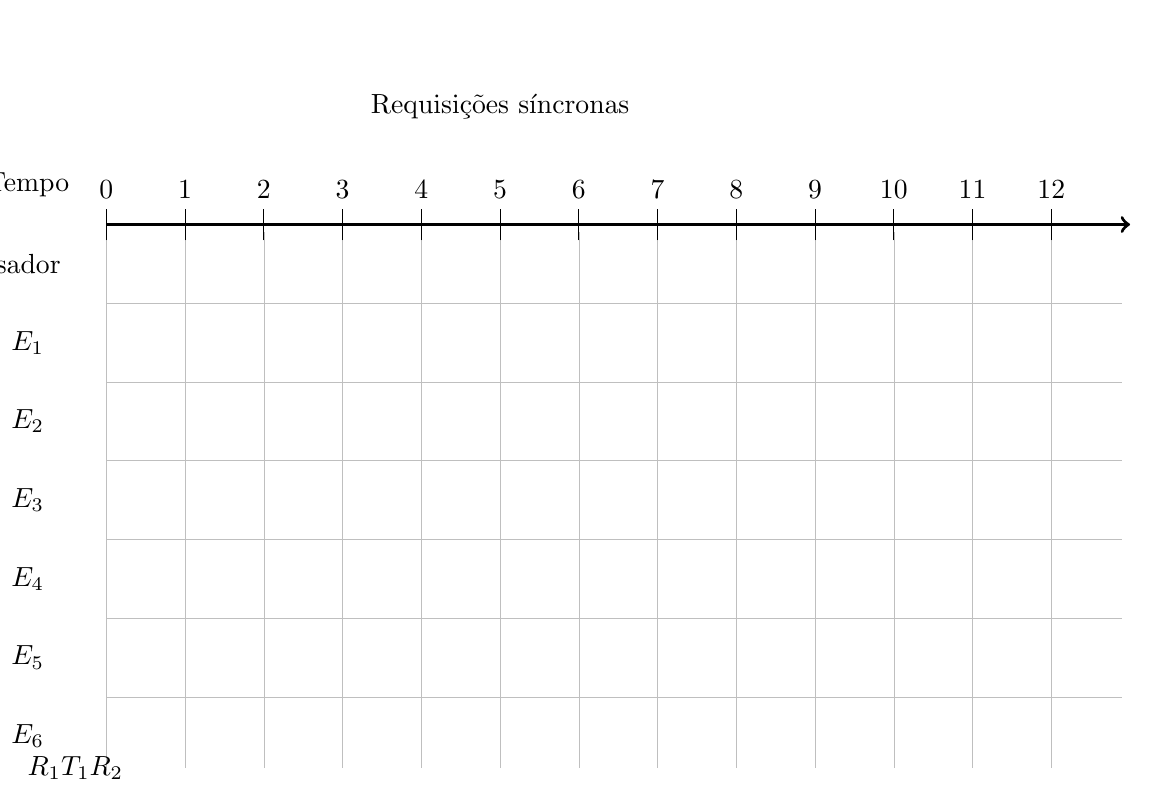
\begin{tikzpicture}
        \useasboundingbox (0,0) rectangle (14,9.5);
        \node at (6, 8.5) {Requisições síncronas};
        \draw[step=1cm,lightgray,very thin] (1,0.1) grid (13.9,6.9);
        \foreach \x in {0,1,2,3,4,5,6,7,8,9,10,11,12}
            \draw ((1cm+\x cm,6.8) -- (1cm+\x cm,7.2) node[anchor=south] {$\x$};
        \draw[very thick,->] (1,7) -- (14,7) node[anchor=south west] {};
        \node at (0,7.5) {Tempo};
        \node at (-0.5,6.5) {Processador};
        \foreach \i in {1,...,6}{
            \node at (0,6.5-\i) {$E_\i$};
        }
        \blocoR{0}{$R_1$}
        \blocoE{1}{1}{6}
        \blocoT{7}{$T_1$}
        \blocoR{8}{$R_2$}
        \blocoE{2}{9}{4}
    \end{tikzpicture}

    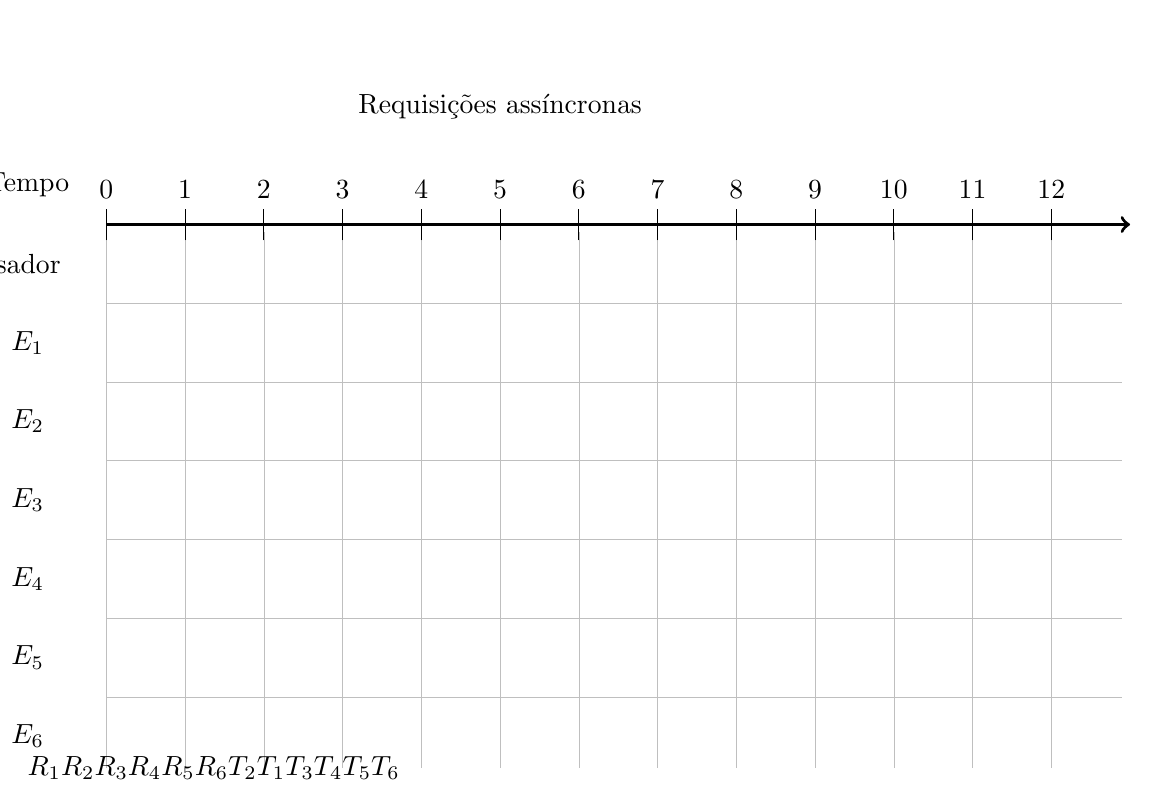
\begin{tikzpicture}
        \useasboundingbox (0,0) rectangle (14,9.5);
        \node at (6, 8.5) {Requisições assíncronas};
        \draw[step=1cm,lightgray,very thin] (1,0.1) grid (13.9,6.9);
        \foreach \x in {0,1,2,3,4,5,6,7,8,9,10,11,12}
            \draw ((1cm+\x cm,6.8) -- (1cm+\x cm,7.2) node[anchor=south] {$\x$};
        \draw[very thick,->] (1,7) -- (14,7) node[anchor=south west] {};
        \node at (0,7.5) {Tempo};
        \node at (-0.5,6.5) {Processador};
        \foreach \i in {1,...,6}{
            \node at (0,6.5-\i) {$E_\i$};
        }
        \foreach \i in {1,2,3,4,5,6}{
            \blocoR{\i-1}{$R_\i$};
        }
        \foreach \i [count=\n] in {2,1,3,4,5,6}{
            \blocoT{\n + 5}{$T_\i$};
        }
        \blocoE{1}{1}{6}
        \blocoE{2}{2}{4}
        \blocoE{3}{3}{4}
        \blocoE{4}{4}{5}
        \blocoE{5}{5}{5}
        \blocoE{6}{6}{5}
    \end{tikzpicture}
    \caption{%
        Comparativo ilustrando como seriam executadas as operações de envio,
        espera e tratamento das requisições enviadas ao servidor de um TJ
        hipotético considerando a obtenção dos dados de 6 processos, enumerados
        como $P_{1...6}$. A sequência das operações estão em passos de tempo
        discretos ordenados da esquerda para direita. A linha ``Processador''
        indica em qual operação o processador está trabalhando em um
        determinado passo de tempo e as linhas $E_{1...6}$ representam uma
        operação de IO relacionada a uma requisição $R_i$, como a espera pela
        resposta do servidor.
        %
        Para cada processo $P_i$, $R_i$ representa a operação de preparo e
        envio da requisição que retornará os dados desse processo, e $T_i$
        representa a operação de tratamento da resposta do servidor do TJ a
        $R_i$ (por exemplo, classificação do processo como
        válido/inválido/inexistente ou reconhecimento de resposta com captcha).
    }
    \label{gra:modelo-temporização-requisições}
\end{figure}

Como forma de evitar sobrecarga dos servidores dos TJs por um excesso de
requisições em um período curto de tempo, evitando possíveis sanções de algum
deles ou mesmo consumo excessivo de memória da máquina cliente devido à
quantidade de objetos das Corrotinas instanciadas para as requisições, foi
implementado um mecanismo limite de requisições simultâneas. O mecanismo
funciona separando os IDs dos processos a serem buscados em ``passos'', em que
cada passo dispara um número fixo de requisições e o próximo passo só é
executado quando todas do atual tiverem sido tratadas. O tamanho (quantidade de
processos por passo) adequado de passo escolhido como padrão foi de
\todofootnote{100 processos}{Escolher valor melhor quando forem apresentados os
resultados}. Resultados de ganhos para diferentes tamanhos de passo estão
expostos na~\todo{\Cref{gra:tempos-tamanhos-de-passo-async}}
(\Cref{chp:Resultados-Experimentais}).

\begin{figure}[htb]
    \caption{Comparação do tempo desprendido por IO e por processamento restrito à CPU.}
    \label{gra:tempo-io-vs-proc}
\end{figure}

Para melhor visualização da implementação,
a~\Cref{lst:requisição-processos-síncrona-e-assíncrona} reproduz, abstraindo as
operações que não dizem respeito à programação assíncrona, o procedimento de
busca por processos respectivamente de forma síncrona e assíncrona.

\begin{listing}[htb]
    \tiny
    \begin{minipage}[t]{0.5\textwidth}
        \begin{minted}[gobble=12,breaklines]{python}
            def fetch_process(
                session: requests.Session,
                url: str,
                id_: str,
            ) -> dict[str, Any]:
                """
                Busca um único processo com o número dado em
                `id_` utilizando a API em `url`, filtrando
                processos por um critério arbitrário (ex:
                se contém um assunto específico).
                """
                response = session.post(
                    url, json={"numProcesso": id_}
                )

                return classify_process(response.json())

            def download_processes(
                url: str,
                ids: list[str],
                sink: Path,  # Onde os processos serão salvos
            ) -> None:
                """Salva todos os processos com determinados IDs em um arquivo JSONL."""
                with requests.Session() as session:
                    for id_ in ids:
                        process = fetch_process(session, id)
                        save_process(process, sink)
        \end{minted}
    \end{minipage}
    \begin{minipage}[t]{0.6\textwidth}
        \begin{minted}[gobble=12,breaklines]{python}
            async def fetch_process(
                session: aiohttp.ClientSession,
                url: str,
                id_: str,
            ) -> dict[str, Any]:
                """
                Busca um único processo com o número dado em
                `id_` utilizando a API em `url`.
                """
                response = requests.post(url, json={"numProcesso": id_})

                return classify_process(response.json(), filter_function)

            async def download_processes(
                url: str,
                ids: list[str],
                sink: Path,  # Onde os processos serão salvos
                step_size: int,  # Número de processos por passo
            ) -> None:
                async with aiohttp.ClientSession() as session:
                    for step_ids in iter_in_steps(ids, step_size):
                        requests = (
                            fetch_process(session, url, step_id)
                            for step_id in step_ids
                        )
                        processes = await asyncio.gather(*requests)

                        for process in processes:
                            save_process(process, sink)
        \end{minted}
    \end{minipage}
    \caption{%
        Reprodução do procedimento de busca por processos de maneira sequencial
        (síncrona, à esquerda) e concorrente/não-bloqueante (assíncrona, à direita).
    }
    \label{lst:requisição-processos-síncrona-e-assíncrona}
\end{listing}


\subsection{\textit{Cache} dos resultados}

\begin{todolist}
    \item Justificar a necessidade de \textit{cache} para os resultados: em
          resumo, requisições, sejam de um mesmo usuário ou de usuários
          diferentes, podem muito bem conter uma intersecção dos processos que
          serão buscados.
    \item Adicionar gráfico comparando o uso da cache para a mesma consulta com
          quando ela é feita com e sem caching.
\end{todolist}

Dado o tempo para realizar uma busca por todos os processos, é inviável que ela
reacesse o servidor dos TJs para cada consulta realizada na ferramenta. A
estratégia para atacar esse problema consiste em guardar os processos
previamente buscados em um banco de dados simples, funcionando como uma
\textit{cache} para os processos já conhecidos. A \textit{cache} acaba sendo
útil também para diferentes requisições em que seus intervalos de números de
processos se interseccionem, visto que a primeira requisição atendida já trará
alguns dos processos da(s) próxima(s), não precisando ser re-buscados por
requisições ao servidor do TJ-RJ já que estarão prontos no banco de dados da
ferramenta. Há também uma vantagem adicional com relação a descoberta de
processos válidos uma vez que, conhecidos todos os processos de um único ano,
não é necessário gastar tempo descobrindo quais números de processos
correspondem a processos reais.

A \textit{cache} foi implementada como um instância de banco de dados
SQLite~\cite{tool:sqlite} com uma única tabela ``Processos'' (reproduzida na
\Cref{tbl:estrutura-tabela-processos}), com a descrição dos valores possíveis
para a coluna \textit{``cache\_state''} descritos
na~\Cref{tbl:valores-coluna-state}. A chave primária da tabela foi escolhida
como o número do processo seguindo a numeração unificada, visto que é uma
informação única a cada processo e, convenientemente, é o parâmetro de busca
utilizado na extração, facilitando a separação de quais processos serão
buscados na \textit{cache} e quais serão requisitados ao servidores dos TJs.

\begin{table}[htb]
    \small
    \centering
    \begin{tabular}{llp{0.6\textwidth}}
        \toprule
        \multicolumn{3}{c}{Processos} \\
        \midrule
        Coluna & Tipo & Descrição \\
        \midrule \\
        *\texttt{id} & text & Número do processo no padrão unificado. \\
        \texttt{cache\_state} & text & Estado atual do processo na \textit{cache}. \\
        \texttt{assunto} & text & Assunto do processo. \\
        \texttt{json} & text & Dados do processo no formato JSON espelhando os campos retornados pela API do ww3. \\
        \bottomrule
    \end{tabular}
    \caption{%
        Definição da tabela SQLite ``Processos'' utilizada para \textit{cache}.
        ``*'' indica que o campo é uma chave primária.
    }
    \label{tbl:estrutura-tabela-processos}
\end{table}

\begin{table}[htb]
    \centering
    \begin{tabular}{lp{0.8\textwidth}}
        \toprule
        Estado & Descrição \\
        \midrule \\
        \texttt{CACHED} & O número do processo é válido e os dados do processo estão na \textit{cache}. \\
        \texttt{INVALID} & O número do processo é inválido (por exemplo, dígitos de validação não conferem pelo algoritmo do TJ). \\
        \texttt{NOT\_CACHED} & O número do processo é válido porém os dados dele não estão na \textit{cache}. Para uso no software, não é registrado na \textit{cache}. \\
        \bottomrule
    \end{tabular}
    \caption{%
        Definição da tabela SQLite ``Processos'' utilizada para \textit{cache}.
        ``*'' indica que o campo é uma chave primária.
    }
    \label{tbl:valores-coluna-state}
\end{table}

Essa separação é uma operação trivial: para saber se um processo deve ou não
ser requisitado aos servidores dos TJs, basta para cada número de processo da
lista de números a serem buscados consultar, na \textit{cache}, se não existe
uma entrada com esse número como valor da chave primária e que o valor de
``cache\_state'' seja ``CACHED''.

Um processo é salvo na \textit{cache} quando

\todo{Falar sobre quando um processo é cacheado e quando não é}

\section{Estratégias adicionais}

\subsection{Filtragem dos resultados}
